\documentclass[tikz, border=5mm]{standalone}
\begin{document}
	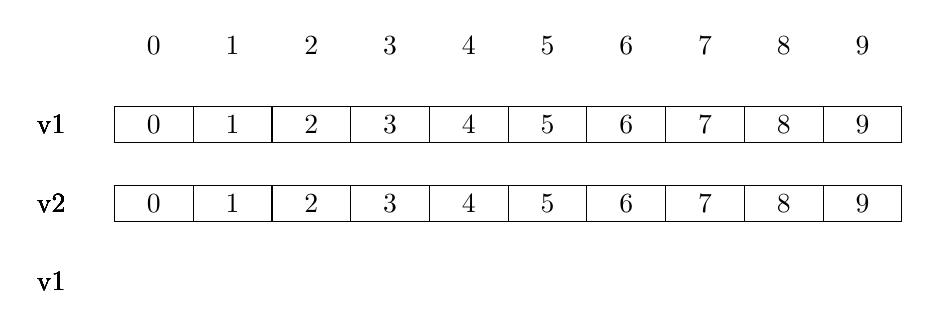
\begin{tikzpicture}
	\foreach \x in {0,...,9} {
		\node at (\x, 0) {\x};
		\foreach \y\lbl in {1/1,2/2,3/1} {
			\node [left] at (-1,-\y) {v\lbl};
			\ifnum\y=3
			\pgfmathtruncatemacro{\result}{2*\x}
			\else
			\node (n\x\y) [draw, minimum width=1cm] at (\x, -\y) {\x};
			\fi
		}
	}
	\end{tikzpicture}
\end{document}